% ---------------- Modelo Trabalho Acadêmico  - Insper ------------------ %

% Este documento contém um modelo para execução de trabalho acadêmico e pode ser utilizado por todos os cursos do Insper que também exijam padronização ABNT.%

%Aqui é utilizada a suíte chamada abnTeX2, a qual formata todo este documento de acordo com as exigências da ABNT, facilitando e automatizando o desenvolvimento da sua monografia em diversas questões (sem mencionar o fato do visual do trabalho ser muito mais agradável esteticamente, se comparado com outros programas de edição de texto). Além disso, foram feitas customizações para atender a certas exigências da Biblioteca Telles, baseando-se no "Manual para elaboração de trabalhos", que pode ser encontrado no site da biblioteca.%

% O abnTeX2 é uma evolução do abnTeX, cujos principais colaboradores G. Weber, L. H. Watter, M. Frasson e outros listados em http://codigolivre.org.br/projects/abntex/, almejavam facilitar a vida dos estudantes e acadêmicos que necessitavam de uma ferramenta para facilmente atender as normas da ABNT em sua produção. Fica aqui a menção aos criadores.%

% Durante o preâmbulo, você vai reparar que este modelo dispõe de notação e ambientes matemáticos que auxiliam na elaboração de um trabalho cujo tema envolva mais matemática. Assim, são definidas diversas notações e ambientes comuns para a Economia (como os símbolos de preferência) de modo a facilitar os autores que foram utilizar isso. No entanto, isso não impede o uso deste modelo por parte daqueles que pouco utilizam, uma vez que a automatização de diversos processos é o ponto mais importante.%

% Este modelo foi feito em cima do disponibilizado no próprio site do abnTeX2 para Monografias e, portanto, compartilha uma estrutura semelhante. Para mais informações visite https://www.abntex.net.br/  %

% A Biblioteca Telles agradece ao alumni Victor Jannuzzi Affonso, que gentilmente cedeu a estrutura desse template para compartilharmos com a comunidade Insper.




% ------- Criação do documento com a classe abntex2 -------- %
\documentclass[
  a4paper, 
  12pt, 
  openany, 
  oneside, 
  brazil,
  % draft
]{abntex2}


% Pacotes utilizados no modelo (nem todos precisam estar presentes para a execução da sua monografia)
\usepackage{times}			% Usa a fonte Times Roman, com compatibilidade matemática
\usepackage[T1]{fontenc}		% Seleção de códigos de fonte.
\usepackage[utf8]{inputenc}		% Codificação do documento (conversão automática dos acentos)
\usepackage{indentfirst}		% Indenta o primeiro parágrafo de cada seção.
\usepackage{color}		        % Controle das cores
\usepackage{graphicx}			% Inclusão de gráficos/figuras.
\usepackage{subcaption}			% Inclusão de subfiguras.
\usepackage{microtype} 			% para melhorias de justificação
\usepackage{amsmath}			% Pacote matemático
\usepackage{amssymb}            % Pacote de símbolos matemáticos
\usepackage[brazil]{babel}      % Pacote para compatibilização com a língua portuguesa
\usepackage{setspace}           % Pacote para espaçamento entre linhas
\usepackage{epstopdf}           % Pacote para conversão em PDF
\usepackage{hyperref}           % Pacote para hyperlinks no documento
\usepackage{amsthm}             % Pacote que define certos ambientes de acordo com a AMS
\usepackage{lipsum}             % Pacote para geração de texto em grego sem sentido (só para preencher as seções)
\usepackage{colortbl}           % Pacote que permite colorir palavras
\usepackage{xcolor}             % Pacote para cores
\usepackage{gensymb}	        % Pacote para símbolos simples
\usepackage{cancel}             % Pacote para mais notação matemática
\usepackage[normalem]{ulem}     % Pacote para underline
\usepackage{booktabs}           % Pacote para tabelas
\usepackage{longtable}
\usepackage{siunitx}            % Pacote para formatação de unidades de medida
\usepackage{amsfonts}           % Pacote para fontes e símbolos matemáticos
\usepackage{lastpage}           % Pacote para tomar a referência da última página
% Pacotes de citações %
\usepackage[brazilian,hyperpageref]{backref}	 % Paginas com as citações na bibl
\usepackage[alf, abnt-emphasize=bf]{abntex2cite}    % Citações padrão ABNT
\usepackage{quoting}                                % Pacote para citações

% Pacotes de gráficos e imagens
\usepackage{adjustbox} % Pacote para ajuste de tamanho de objetos
\usepackage{pgfplots} % Pacote para criação de gráficos
\usepackage{pdfpages} % Pacote para inclusão de arquivos PDF
\usepackage{anyfontsize} % Pacote para especificação de tamanhos de fonte arbitrários

\pgfplotsset{compat=newest}
\usepgfplotslibrary{statistics}
\usepgfplotslibrary{fillbetween}
\usetikzlibrary{decorations.markings,decorations.pathmorphing}
\usetikzlibrary{intersections}


\pgfplotsset{
    standard/.style={
    axis line style = thick,
    enlargelimits,
    axis x line=middle,
    axis y line=middle,
    enlarge x limits=0.15,
    enlarge y limits=0.15,
    width = \linewidth
    }
}

\newcolumntype{d}{S[ input-open-uncertainty=, input-close-uncertainty=, parse-numbers = false, table-align-text-pre=false, table-align-text-post=false ]} %Tabela R modelsummary

% \usepackage[table,xcdraw]{xcolor}

% --------------- Definições e notações matemáticas usadas no texto -----------------%

% Conjuntos de números naturais, racionais e reais
\def\N{\mathbb{N}}
\def\Q{\mathbb{Q}}
\def\R{\mathbb{R}}

% Símbolos letras maiúsculas caligráficas
\def\A{\mathcal{A}}
\def\B{\mathcal{B}}
\def\C{\mathcal{C}}
\def\D{\mathcal{D}}
\def\E{\mathcal{E}}
\def\F{\mathcal{F}}
\def\H{\mathcal{H}}
\def\I{\mathcal{I}}
\def\L{\mathcal{L}}
\def\P{\mathcal{P}}
\def\R{\mathbb{R}}
\def\S{\mathcal{S}}
\def\T{\mathbb{T}}
\def\X{\mathcal{X}}
\def\Y{\mathcal{X}}
\def\W{\mathcal{Z}}

% Símbolos específicos
\def\pf{\succcurlyeq}
\def\ps{\succ}
\def\ind{\sim}
\def\inc{\not \gtrless}
\def\pft{\preccurlyeq}
\def\pst{\prec}
\newcommand{\incomparavel}{\succ\kern-0.45cm \prec}

%%% Símbolos lógicos
\def\oulog{\vee}
\def\elog{\wedge}
\def\implica{\Rightarrow}
\def\eeq{\Leftrightarrow}

% Ambientes - Teoremas, etc. - A numeração de cada ambiente no texto é feita de acordo com o ambiente escolhido.
\newtheorem{axiomas1}{Axioma}
\newtheorem{teo1}{Teorema}
\newtheorem{lema1}{Lema}
\newtheorem{defi1}{Definição}
\newtheorem{ex1}{Exemplo}
\newtheorem{prop1}{Proposição}




% ------------------ Configuração e customização dos pacotes ---------------------- %

% Configurações do pacote backref
% Usado sem a opção hyperpageref de backref
\renewcommand{\backrefpagesname}{}
% Texto padrão antes do número das páginas
\renewcommand{\backref}{}
% Define os textos da citação
\renewcommand*{\backrefalt}[4]{}%


% Customização da capa
\renewcommand{\imprimircapa}{%
    \begin{capa}%
    \center{\ABNTEXchapterfont\large\imprimirinstituicao}
    
    \vspace*{\fill}
    
    \center{\ABNTEXchapterfont\large\imprimirautor}
    
    \vspace*{\fill}
    {\ABNTEXchapterfont\bfseries\LARGE\imprimirtitulo}
    \vspace*{\fill}
    
    {\large\imprimirlocal}
    \par
    {\large\imprimirdata}
\vspace*{1cm}
\end{capa}
}


% Customização do cabeçalho
\makepagestyle{tccinsper}
  %cabeçalhos
  \makeevenhead{tccinsper} %%pagina par
     {}
     {}
     {\thepage}
       \makeoddhead{tccinsper} %%pagina com oneside
     {}
     {}
     {\thepage}

% Customização dos hiperlinks
\definecolor{Lgray}{RGB}{207,207,207}
\definecolor{black}{RGB}{0,0,0}
\makeatletter
\hypersetup{
                % pagebackref=true,
		pdftitle={\@title},
		pdfauthor={\@author},
    	        pdfsubject={\imprimirpreambulo},
	        pdfcreator={LaTeX with abnTeX2},
		% pdfkeywords={abnt}{latex}{abntex}{abntex2}{relatório técnico},
		colorlinks=true,       		% false: boxed links; true: colored links
                % colorlinks=false,
                linkcolor=black,          	% color of internal links
                citecolor=black,        		% color of links to bibliography
                filecolor=magenta,      		% color of file links
                urlcolor=black,
                bookmarksdepth=4
}
\makeatother


% Configuração dos espaçamentos entre linhas e parágrafos

% O tamanho do parágrafo é dado por:
\setlength{\parindent}{1.3cm}

% Controle do espaçamento entre um parágrafo e outro:
\setlength{\parskip}{0.2cm}  % tente também \onelineskip

% Compila o indice
\makeindex


% Mais alguns comandos personalizados
\newcommand*\rfrac[2]{{}^{#1}\!/_{#2}}
\renewcommand{\arraystretch}{1.3} 			% Espaçamento na tabela
\newcommand{\volume}{\mathop{\ooalign{\hfil$V$\hfil\cr\kern0.08em--\hfil\cr}}\nolimits} % Símbolo V cortado
\newcommand\rlArrow[1]{$\color{red}{abc \rightarrow} #1 \color{blue}{\leftarrow} abc$}


% Informações de dados para CAPA
\autor{Gustavo Theil}
\titulo{Miopia ou controle? Análise da eficiência dos instrumentos regulatórios urbanos para determinação de densidade habitacional}
\instituicao{
  %
  Insper Instituto de Ensino e Pesquisa

  Ciências Econômicas
  }
\local{São Paulo - SP}
\data{2024}

% Informações de dados para FOLHA DE ROSTO

\autor{Gustavo Theil}
\titulo{Miopia ou controle? Análise da eficiência dos instrumentos regulatórios urbanos para determinação de densidade habitacional}
\orientador{Adriano Borges Costa}
\local{São Paulo - SP}
\data{2024}

\preambulo{Iniciação Científica}


% ------------------------------------------------------------------------------ %
% --------------------------- Início do documento ------------------------------ %
% ------------------------------------------------------------------------------ %
\begin{document}

% Retira espaço extra obsoleto entre as frases.
\frenchspacing

% ------------------------------------------------------------------------ %
%                          ELEMENTOS PRÉ-TEXTUAIS
% ------------------------------------------------------------------------ %
\pretextual


% Capa e Folha de Rosto
\imprimircapa
\imprimirfolhaderosto

% Configuração da ficha catalográfica
\begin{fichacatalografica}
    \vspace*{15cm} % Posição vertical
    \hrule % Linha horizontal
    \begin{center} % Minipage Centralizado
    \begin{minipage}[c]{12cm} % Largura
    
    \imprimirautor
    
    \hspace{0.5cm} \imprimirtitulo / \imprimirautor. -
    \imprimirlocal: \imprimirdata

    \hspace{0.5cm} \pageref{LastPage} p.

\hspace{0.5cm}
\parbox[t]{\textwidth}{\imprimirtipotrabalho: \ \imprimirinstituicao, \imprimirdata.}\\

\hspace{0.5cm} \imprimirorientadorRotulo \ \imprimirorientador

    \hspace{0.5cm}
1. Economia Urbana
2. Política pública
I. \imprimirautor.
II. \imprimirtitulo.
    \end{minipage}
    \end{center}
    \hrule
\end{fichacatalografica}

\clearpage
% % Configuração da folha de aprovação
% \begin{folhadeaprovacao}

%   \begin{center}
%     {\ABNTEXchapterfont\large\imprimirautor}

%     \vspace*{\fill}\vspace*{\fill}
%     \begin{center}
%       \ABNTEXchapterfont\bfseries\Large\imprimirtitulo
%     \end{center}
%     \vspace*{\fill}
    
%     \hspace{.45\textwidth}
%     \begin{minipage}{.5\textwidth}
%         \imprimirpreambulo
%     \end{minipage}%
%     \vspace*{\fill}
%    \end{center}
        
%     \vspace*{\fill}
        
%     \begin{center}
%       \ABNTEXchapterfont\bfseries\large{Banca examinadora}
%     \end{center}
        
%     \vspace*{\fill}
%    %Trabalho aprovado. \imprimirlocal, x de x de x:

%    \assinatura{\textbf{\imprimirorientador} \\ Orientador(a)} 
%    \assinatura{\textbf{Professor} \\ Examinador(a)}
%    %\assinatura{\textbf{Professor} \\ Examinador(a)}
%    %\assinatura{\textbf{Professor} \\ Examinador(a)}
%    %\assinatura{\textbf{Professor} \\ Examinador(a)}
      
%    \begin{center}
%     \vspace*{0.5cm}
%     {\large\imprimirlocal}
%     \par
%     {\large\imprimirdata}
%     \vspace*{1cm}
%   \end{center}
  
% \end{folhadeaprovacao}

% \begin{agradecimentos}
% \lipsum[1-2]
% \end{agradecimentos}


% Resumo e abstract
% Resumo em português
\setlength{\absparsep}{18pt} % ajusta o espaçamento dos parágrafos do resumo
\begin{resumo}

O Plano Diretor Estratégico (PDE 2014) do município de São Paulo tem como um dos principais objetivos gerar adensamento populacional nas áreas mais desejáveis. 

% O escopo desta pesquisa é compreender o funcionamento das forças de mercado e indentificar se os instrumentos de regulação são capazes de gerar os incentivos almejados pelo PDE. 

O escopo desta pesquisa é

As estimativas apontam que cerca de metade da cidade não responde aos incentivos, já que não está registrada no Cadastro Imobiliário Fiscal e portanto se encontra em situação informal. Para a outra metade, identificou-se que entre os instrumentos utilizados para a regulação, a cota parte se demonstrou a mais efetiva para definir a densidade populacional, seguida pelo Coeficiente de Aproveitamento (CA). O número de pavimentos se mostrou irrelevante. 

Palavras-chave: Economia Urbana, Política Pública, Plano Diretor
\end{resumo}

% Resumo em inglês
\begin{resumo}[Abstract]
 \begin{otherlanguage*}{english}

  One of the main goals of the Strategic Master Plan (2014) of São Paulo is generate population density in the most desirable areas. The scope of this research is to understand the market forces and to identify whether regulatory instruments are capable of generating the desired outcomes. Estimates indicate that about half of the city does not respond to incentives, as it is not registered in the Fiscal Real Estate Registry and therefore is in an informal status. For the other half, it was identified that among the instruments used for regulation, the ``cota parte'', or \textit{shared quota} proved to be the most effective in defining population density, followed by the floor area ratio (FAR). The number of floors was found to be irrelevant.

Keywords: Urban Economics, Public Policy, Master Plan
 \end{otherlanguage*}
\end{resumo}


% Insere o sumário automático
\pdfbookmark[0]{\contentsname}{toc}
\tableofcontents*
\cleardoublepage


\textual
\pagestyle{tccinsper} %Define o estilo da página utilizado

\chapter{Introdução}

\subsection*{\textbf{Por que cidades existem?}}

Para Bauman, cidades são lugares de oportunidades e são movidas por ``newcomers'', pessoas que não são originalmente do lugar e são estranhos à sua realidade. Quando essas pessoas chegam nas cidades, elas apresentam novas perspectivas sobre problemas antigos e suas formas de pensar geralmente conflitam com tranquilidade consequente da familiaridade e convivência dos residentes bem estabelecidos. Apesar disso poder gerar incômodo aos nativos, é para o bem deles e da cidade que suas formas de ser sejam questionadas e desafiadas pelos estranhos. Para o autor, esse estado de inquietude e permanente sentimento de ``ser estrangeiro'' é o que leva as pessoas e a cidade a buscar reflexão, debate e inovação \cite{bauman2003city}.

Para Jane Jacobs, uma característica que determina o sucesso de uma cidade é sua vitalidade. A autora defendia que a vida na cidade depende fortemente das dinâmicas sociais, das interações cotidianas de seus residentes. Para Jacobs, a cidade proporciona interações nos espaços públicos -- onde a vida urbana efetivamente acontece -- e possibilita que as pessoas se conectem, encontrem, colaborem e prosperem juntas. Ela valorizava a diversidade, densidade e a mistura de usos do solo urbano, argumentando que a presença de uma variedade de estabelecimentos comerciais, residenciais e culturais em uma mesma área promove a interação entre diferentes grupos sociais e estimulava a criatividade e a inovação \cite{jacobs1961death}.

Do ponto de vista econômico, o triunfo da cidade se encontra nos benefícios de aglomeração e adensamento. Economias de aglomeração permitem que firmas diferentes escolham ficar geograficamente próximas umas das outras e encontrem benefício econômico ao reduzirem seus custos e aumentarem a produtividade. Jan Brueckner, em \textit{Lectures on Urban Economics}, delimita no capítulo 1 o racional econômico da existência de cidades, que se divide em quatro principais componentes.

A aglomeração tecnológica $(i)$ aumenta a produtividade dos trabalhadores, na medida em que os empregos são mais concentrados e há ``transbordamento'' de conhecimento entre as firmas da região. Além disso, uma oferta maior e mais diversa de trabalho, causa maior competitividade e eficiência na escolha da pessoa certa para cada cargo. Aglomerações pecuniárias $(ii)$ reduzem os custos das firmas, sem alterar sua produtividade. Com maior demanda por serviços como segurança, limpeza, contratação e advocacia, estes mercados se desenvolvem, tornam-se mais competitivos, eficientes e baratos. Inclusive, há serviços especializados de nicho, que podem estar disponíveis e acessíveis apenas em grandes centros urbanos. Aglomeração de varejo $(iii)$ traz ganhos para os consumidores e comerciantes. Quando o comércio está aglomerado, o consumidor pode escolher entre mais opções e se desloca menos entre seus destinos caso queria comprar mais de um item. Dessa forma, os consumidores ganham e os comerciantes também, visto que com mais consumidores e maior fluxo, maiores as vendas. Por fim, o custo de transporte $(iv)$ é um dos fatores que mais mudam quando há densidade. A redução do custo de transporte, que pode ser considerada uma economia de aglomeração pecuniária, acontece não apenas para os trabalhadores, que se deslocam menos às oportunidades de emprego, mas também às firmas que gastam menos transportando seus bens e serviços \cite{brueckner2011lectures}.

Nesse sentido, se aglomeração e densidade trazem benefícios, uma cidade bem sucedida é uma cidade que ao longo do tempo tende a se adensar cada vez mais. Entretanto, uma pergunta relevante é se as forças de aglomeração atuam sozinhas ou se precisam de incentivos e regulação. Os modelos de economia urbana demonstram que as próprias forças de mercado agem de forma a incentivar o adensamento, mas há fatores que podem atuar na direção contrária também \cite{brueckner2011lectures} -- mais detalhes serão discutidos na Seção \ref{sec:micro}. Nessa perspectiva, a função das instituições seria de intervir de forma a combater essas forças, apoiando o adensamento. 

Por outro lado, Edward Glaeser em \textit{Triumph of the City} discute alguns desafios encontrados pela regulamentação e incentivos criados pelas insituições. Segundo o autor, muitas vezes a regulamentação apresenta procedimentos lentos e burocráticos, e acaba gerando decisões focadas em fatores que se sobrepõem o adensamento na escala de prioridades. Inclusive, o que Glaeser propõe é criar impostos \textit{à la} Coase, de forma que os incentivos se alinhem para uma cidade mais densa, ainda compensando pelos seus possíveis malefícios. 

Ronald Coase reconhece natureza recíproca do problema do custo social, no caso em que A causa malefícios a B, mas B também causa malefícios a A. Isso se aplica a um exemplo em que uma empresa (A) quer construir um prédio, mas a comunidade local não quer ser perturbada mudanças na região. Caso a empresa (A) siga com a construção, a comunidade local (B) será prejudicada, mas se a construção for barrada, a empresa (A) também sofrerá e menos oferta habitacional e empregos serão gerados. Coase propõe uma forma de pensar que leva em conta não apenas a ponderação de qual malefício é maior, mas também a compensação da parte que sai prejudicada de um eventual acordo. Dessa forma, é sempre feita a escolha que maximize o bem-estar social, sem causar distorções nas escolhas, ainda compensando a parte prejudicada \cite{coase2013problem}.

\begin{quotation}
   ``Primeiro, as cidades devem substituir seus longos e incertos procedimentos de licenciamento com um simples sistema de taxação. Se prédios altos criam custos ao bloquear vistas ou luz, então faça uma estimativa razoável desses custos e cobre o construtor de acordo. Se certas atividades são nocivas aos vizinhos, então devemos estimar o custo social e cobrar os construtores por eles, assim como devemos cobrar motoristas pelos custos de gerar engarrafamentos. Esses impostos podem então ser dados às pessoas que estão sendo impactadas, como os vizinhos que perderam a iluminação por um novo prédio que obstrui sua vista.'' \cite{glaeser2011triumph}

\end{quotation}

\subsection*{\textbf{Regulamentação em São Paulo}}

Atualmente em São Paulo, os mecanismos de regulação são principalmente definidos pelo atual Plano Diretor Estratégico de SP \cite[PDE]{PDE}. No código da lei do PDE, entre os 17 objetivos estabelecidos, ao menos nove estão relacionados a estratégias de adensamento urbano \cite{lima2021alem}. A ideia principal do plano é direcionar o adensamento para áreas capazes de admitir um grande volume de habitantes, principalmente no entorno de infraestruturas de transporte de alta capacidade.

O PDE institui uma variedade de instrumentos para gerar esse adensamento, alguns atuando sobre empreendimentos já existentes, e outros para os novos também. O artigo 96 do PDE estabelece que ``os imóveis não edificados, subutilizados e não utilizados são sujeitos ao parcelamento, edificação e utilização compulsórios'', de forma a passar a exercer sua função social dentro de um prazo estabelecido. Existem, inclusive, dispositivos para lidar especificamente com imóveis com este perfil em áreas que dispõem das características apropriadas para um maior adensamento, como é o caso das ZEIS 3:

\begin{quotation}
    ``ZEIS 3 são áreas com ocorrência de imóveis ociosos, subutilizados, não utilizados, encortiçados ou deteriorados localizados em regiões dotadas de serviços, equipamentos e infraestruturas urbanas, boa oferta de empregos, onde haja interesse público ou privado em promover Empreendimentos de Habitação de Interesse Social''

    \raggedleft Art. 45 do PDE \cite{PDE}
\end{quotation}

Para a regulação dos novos empreendimentos, há três principais dispositivos. O primeiro deles é o gabarito, que determina a altura máxima, em metros, dos imóveis. Outro instrumento é o coeficiente de aproveitamento (CA), que determina quantas vezes a área do lote pode ser construída. Se o CA é básico (CA = 1), e o lote possui 1.000m$^2$, então pode ser construído um empreendimento que distribui estes 1.000m$^2$ em uma quantidade qualquer de andares que respeite o gabarito. Se o CA for 2, significa que para o mesmo lote, podem ser distribuídos 2.000m$^2$ em \textit{n} andares. Por fim, a cota parte é a cota máxima de terreno por unidade habitacional e determina o número mínimo de unidades habitacionais do terreno. Para calcular a cota parte, basta dividir o lote pelo número de unidades, resultando na cota do terreno ocupada por cada unidade habitacional. Dessa forma, o número mínimo de unidades habitacionais é dado pela Equação \ref{eq:cotaparte}, na qual $A_t$ representa a área do lote e $Q$ a cota parte.

\begin{equation}
    N_{min} = \frac{\text{CA}_{\text{utilizado}}}{\text{CA}_{max}}\cdot \frac{A_t}{Q}
    \label{eq:cotaparte}
\end{equation}

No PDE, foram estabelecidos diferentes níveis de CA na cidade, a depender dos objetivos que se tem em relação à região, como é possível observar na Figura \ref{fig:CA}. Nas regiões de preservação ambiental, por exemplo, o CA é de 0.1, o menor da cidade, enquanto nas áreas do entorno de equipamentos de transporte pública de alta capacidade, (EETUs), o CA chega a 4. Com isso, o adensamento é direcinado às áreas que são aptas a receber mais habitantes.

\begin{figure}[h]
    \caption{Coeficientes de aproveitamento (CA) na cidade}
    \label{fig:CA}
    

    \caption*{\raggedright \textbf{Macroáreas}}
    \begin{subfigure}{.9\textwidth}
        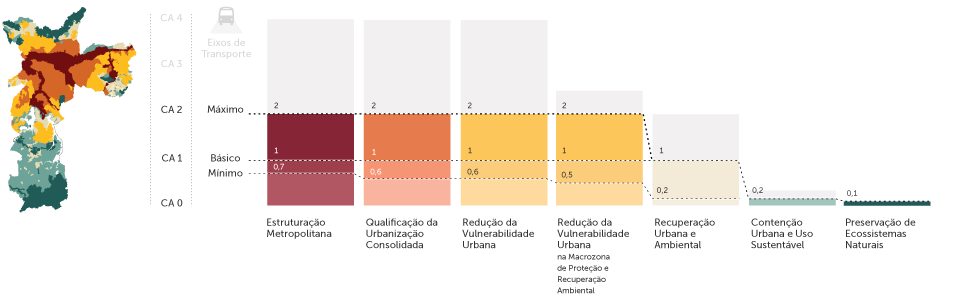
\includegraphics[width = \textwidth]{imagens/CA_macroareas.png}
    \end{subfigure}

    \caption*{\raggedright \textbf{Eixos de Estruturação da Transformação Urbana (EETU)}}
    \begin{subfigure}{.9\textwidth}
        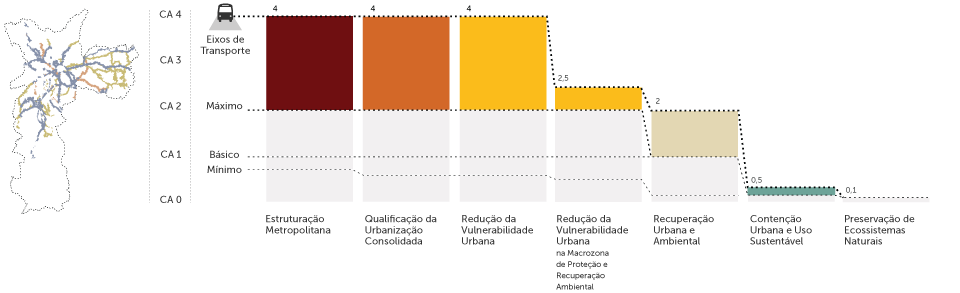
\includegraphics[width = \textwidth]{imagens/CA_eixos.png}
    \end{subfigure}
    \caption*{Fonte: \url{https://gestaourbana.prefeitura.sp.gov.br/marco-regulatorio/plano-diretor/entenda-o-projeto-de-lei-68813/}}
\end{figure}

Da mesma forma, existem parâmetros para a cota parte na cidade, a depender da localização. Nas Macrozonas de Estruturação e Qualificação Urbana, por exemplo, a cota parte apontada na Equação \ref{eq:cotaparte} como $Q$ equivale a 20. Em termos práticos, isso significa que um lote de 1.000m$^2$ hipotético deve apresentar no mínimo 50 unidades habitacionais. Este valor não é incrementado por um aumento do CA, mas pode decrescer se o CA escolhido pelo projeto seja menor do que o CA máximo da região.

Nesse sentido, não existe exatamente um dispositivo que determine a densidade populacional em si. Isso pode levar a um cenário em que o mercado está fracamente regulado, implicando que a densidade não está sendo efetivamente decidia pelo PDE. Apesar de haver um número mínimo de unidades habitacionais, estas não necessariamente se traduzem em população, dado que ao mesmo tempo que pode abrigar uma única pessoa, também pode abrigar uma família com diversos membros. Além disso, este valor mínimo não é afetado pela verticalização do imóvel, então imóveis com um CA maior não são obrigados a terem mais unidades habitacionais.

\subsection*{\textbf{O problema}}

Levando em consideração que um dos principais objetivos do PDE é estimular o adensamento de determinadas áreas, é importante avaliar se os instrumentos de regulação que estão disponíveis para alcançar este objetivo são eficientes. Em outras palavras, é crucial entender se os 3 components expostos (CA, cota parte e gabarito) são suficientes para determinar a densidade populacional que um novo empreendimento vai gerar. 

Caso estes instrumentos apontados não sejam eficientes em determinar a densidade, o nível de adensamento estaria sendo decidido pelo mercado. Entretanto, o que é importante notar é que o mercado sempre busca maximizar seus lucros, o que não necessariamente reflete em maior densidade populacional. Do ponto de vista teórico, é importante compreender quais elementos estão envolvidos nas escolhas das firmas na oferta de unidades de habitação, que será uma discussão da Seção \ref{sec:micro}.

Na Seção \ref{sec:emp}, será avaliado se estes instrumentos determinam a densidade demográfica. Para tanto, serão usados os dados do IPTU para calcular os indicadores utilizados na regulação e os dados do Censo de 2022, para identificar a densidade demográfica da região. Caso os indicadores sejam suficientes para explicar a densidade, significa que o PDE consegue definir a densidade usando os instrumentos previstos na lei. Caso contrário, a densidade populacional está sendo efetivamente decidida via mercado, não estando necessariamente alinhada com os objetivos do Plano para a cidade.

\chapter{Teórico}
\label{sec:micro}

Na literatura microeconômica há diversos modelos que tentam compreender as dinâmicas econômicas da cidade. Utilizando premissas formais e provas matemáticas, é possível resolver o modelo para algumas variáveis endógenas, como preço por metro quadrado na cidade, uso do solo, densidade populacional, entre outros \cite{papageorgiou2012essay, fujita1989urban}. A seguir será apresentado o modelo simplificado desenvolvido em \cite{brueckner2011lectures}, com o foco na variável densidade habitacional. O objetivo é compreender como o mercado se comportaria sem a intervenção da regulamentação e qual seria o seu impacto na variável resposta.

O modelo microeconômico começa com premissas simplificadoras fortes, mas que podem ser flexibilizadas na medida que algum componente merece ser discutido. Em sua primeira versão, a cidade é um círculo no qual todos os empregos se encontram no centro, as pessoas se deslocam uma distância ($x$) para trabalhar, o custo de transporte por distância é ($t$) e todos os moradores apresentam a mesma renda ($y$). A renda disponível é definida pela renda subtraída dos custos de transportes ($T=tx$). Por simplificação também, em cada unidade habitacional habita apenas uma pessoa. Nesse sentido, a densidade ($D$) é definida pelo número de unidades habitacionais por área.

Como o sistema está sempre em equilíbrio, todos os moradores apresentam a mesma utilidade em morar em cada ponto da cidade. Caso um lugar fosse melhor de morar, todos iriam querer se mudar para essa localização, aumentando seu preço ($p$). A função de utilidade dos cidadãos é composta por consumo de habitação ($q$) e outros bens, apelidados por pão, ($c$)\footnote{Por fins de simplificação, o preço do pão (outros bens) foi definido como unitário.}, de forma que toda sua renda disponível será gasta com estes bens, então $y-tx=c+pq$. Para o consumidor, sempre é melhor consumir unidades habitacionais maiores e mais pão, ou seja, quanto maior $p$ e $c$, maior sua utilidade. Dessa forma, quanto mais próximo do centro, e, portanto, um menor $x$, maior pode ser o gasto com $q$ e $c$.

Analogamente, os produtores também apresentam lucro igual para produção imobiliária em todos os pontos da cidade. Se algum lugar na cidade lucrasse mais do que outro, as firmas buscariam produzir lá e, portanto, seu preço reduziria com a expansão de oferta, equilibrando o sistema. Os produtores apresentam uma função de produção que depende do preço ($r$) da terra ($l$) e do custo ($i$) da verticalização ($N$). Se construir um novo andar em um terreno existente for mais barato que comprar um novo terreno, a incorporadora decidirá por verticalizar, mas a cada novo andar construído, o próximo apresentará um custo maior.

Com o modelo construído, agora é possível resolvê-lo de forma a descobrir o preço do metro quadrado na cidade. Na Figura \ref{fig:micro} é possível observar o que acontece com o preço por metro quadrado ($p$) na medida em que aumenta a distância ao centro ($x$). Como a renda é constante na cidade e os preços por metro quadrado são maiores no centro, os habitantes no centro conseguem comprar apartamentos menores. Dessa forma a densidade habitacional apresenta o mesmo comportamento do que o preço do metro quadrado: na medida em que aumenta $x$, $D$ reduz.

\begin{figure}[h]
    \centering
    \caption{Curva de preço por metro quadrado}
    \begin{subfigure}{.6\linewidth}
        \begin{tikzpicture}

    \begin{axis}[standard,
        xtick={0},
        ytick={0},
        xticklabels = {},
        yticklabels = {},
        samples=100,
        xlabel={Distância ao centro ($x$)},
        ylabel={\$},
        xmin=0,xmax=2,
        ymin=0,ymax=1,
        y label style={anchor=east},
        x label style={anchor=north},
    ]
    
\addplot[name path=F,domain={0:2}]{e^(-x)} node[pos=1] (point) {};
\node [right] at (point) {$p$};



    
\end{axis}
\end{tikzpicture}
    \end{subfigure}
    \label{fig:micro}
\end{figure}

Portanto, com essas premissas e resultados, não é necessária a intervenção do governo para regulamentar a densidade, visto que as próprias forças de mercado adensam as regiões centrais. Dessa forma, regulamentações podem mais gerar peso morto, ineficiência e burocracia. Entretanto, algumas das premissas do modelo são tão fortes, que o tornam descolado da realidade. Inclusive, o efeito da distância pode ser ambíguo na densidade a depender de algumas premissas. 
% Um exemplo disso é quando se incorpora no modelo níveis de renda diferentes.

Suponha uma cidade na qual os habitantes possuem mais de uma opção de meio de transporte. Os ricos, por exemplo, se deslocam de carro e os pobres, de ônibus. Como o carro apresenta um custo mais alto, esse grupo vai valorizar mais morar em regiões centrais, visto que o efeito da distância ($x$) em sua renda disponível é maior. Com este novo cenário, o quanto cada grupo está disposto a pagar pelo metro quadrado muda do cenário da Figura \ref{fig:micro} para a Figura \ref{fig:micro-2}, na qual se observa um padrão de segregação espacial dos dois grupos. Os ricos, que habitam o centro, possuem um maior poder aquisitivo, então vão consumir apartamentos maiores. Como consequência, têm-se que com essas novas premissas, a densidade habitacional no centro já não é mais tão grande.

\begin{figure}[h]
    \centering
    \caption{Curva de preço por metro quadrado com dois grupos}
    \begin{subfigure}{.6\linewidth}
        \begin{tikzpicture}

    \begin{axis}[standard,
        xtick={0},
        ytick={0},
        xticklabels = {},
        yticklabels = {},
        samples=100,
        xlabel={Distância ao centro ($x$)},
        ylabel={\$},
        xmin=0,xmax=2,
        ymin=0,ymax=1,
        y label style={anchor=east},
        x label style={anchor=north},
    ]
    
\addplot[name path=F,domain={0:2}]{e^(-x)} node[pos=1] (point1) {};
\node [right] at (point1) {$p_R$};

\addplot[name path=G,domain={0:2}]{0.5 * e^(-0.5*x) + .1} node[pos=1] (point2) {};
\node [right] at (point2) {$p_P$};

\path [name intersections={of=G and F, by = intersec}]; 
\draw[dashed] (intersec) -- (intersec|-{axis cs:0,0});

    
\end{axis}
\end{tikzpicture}
    \end{subfigure}
    \label{fig:micro-2}
\end{figure}


% Supondo agora uma cidade que possui dois grupos de renda, os ricos e os pobres. As outras premissas se mantém. Agora, se tanto os pobres quanto os ricos estiverem competindo pela mesma unidade habitacional, sempre vencerá quem consegue pagar o maior preço. Para determinar a localização que cada grupo se encontra na cidade, é importante comparar as curvas de preço, como da Figura \ref{fig:micro}, e analisar para cada parte da cidade, quem está disposto a pagar mais pela unidade habitacional.

% Várias hipóteses de como essas curvas se comportam podem surgir, a depender de como o componente renda é incorporado no modelo. Uma que é razoável para o Brasil


\chapter{Empírico}
\label{sec:emp}

\section{Dados}

Para compreender o perfil geográfico da distribuição populacional de São Paulo foram utilizados os dados preliminares do Censo de 2022, feito pelo IBGE. Segundo o levantamento, a atual população do município de SP se encontra em 11.451.999 de habitantes, dividios em 4.996.529 de domicílios, dos quais apenas 4.316.336 estão ocupados. Na Figura \ref{fig:populacao} é possível observar quais são as áreas mais densas da cidade. A densidade foi calculada através da população no setor censitário dividida pela sua área.


\begin{figure}[h]
    \centering
    \caption{Densidade populacional em São Paulo por setor censitário (Censo 2022)}
    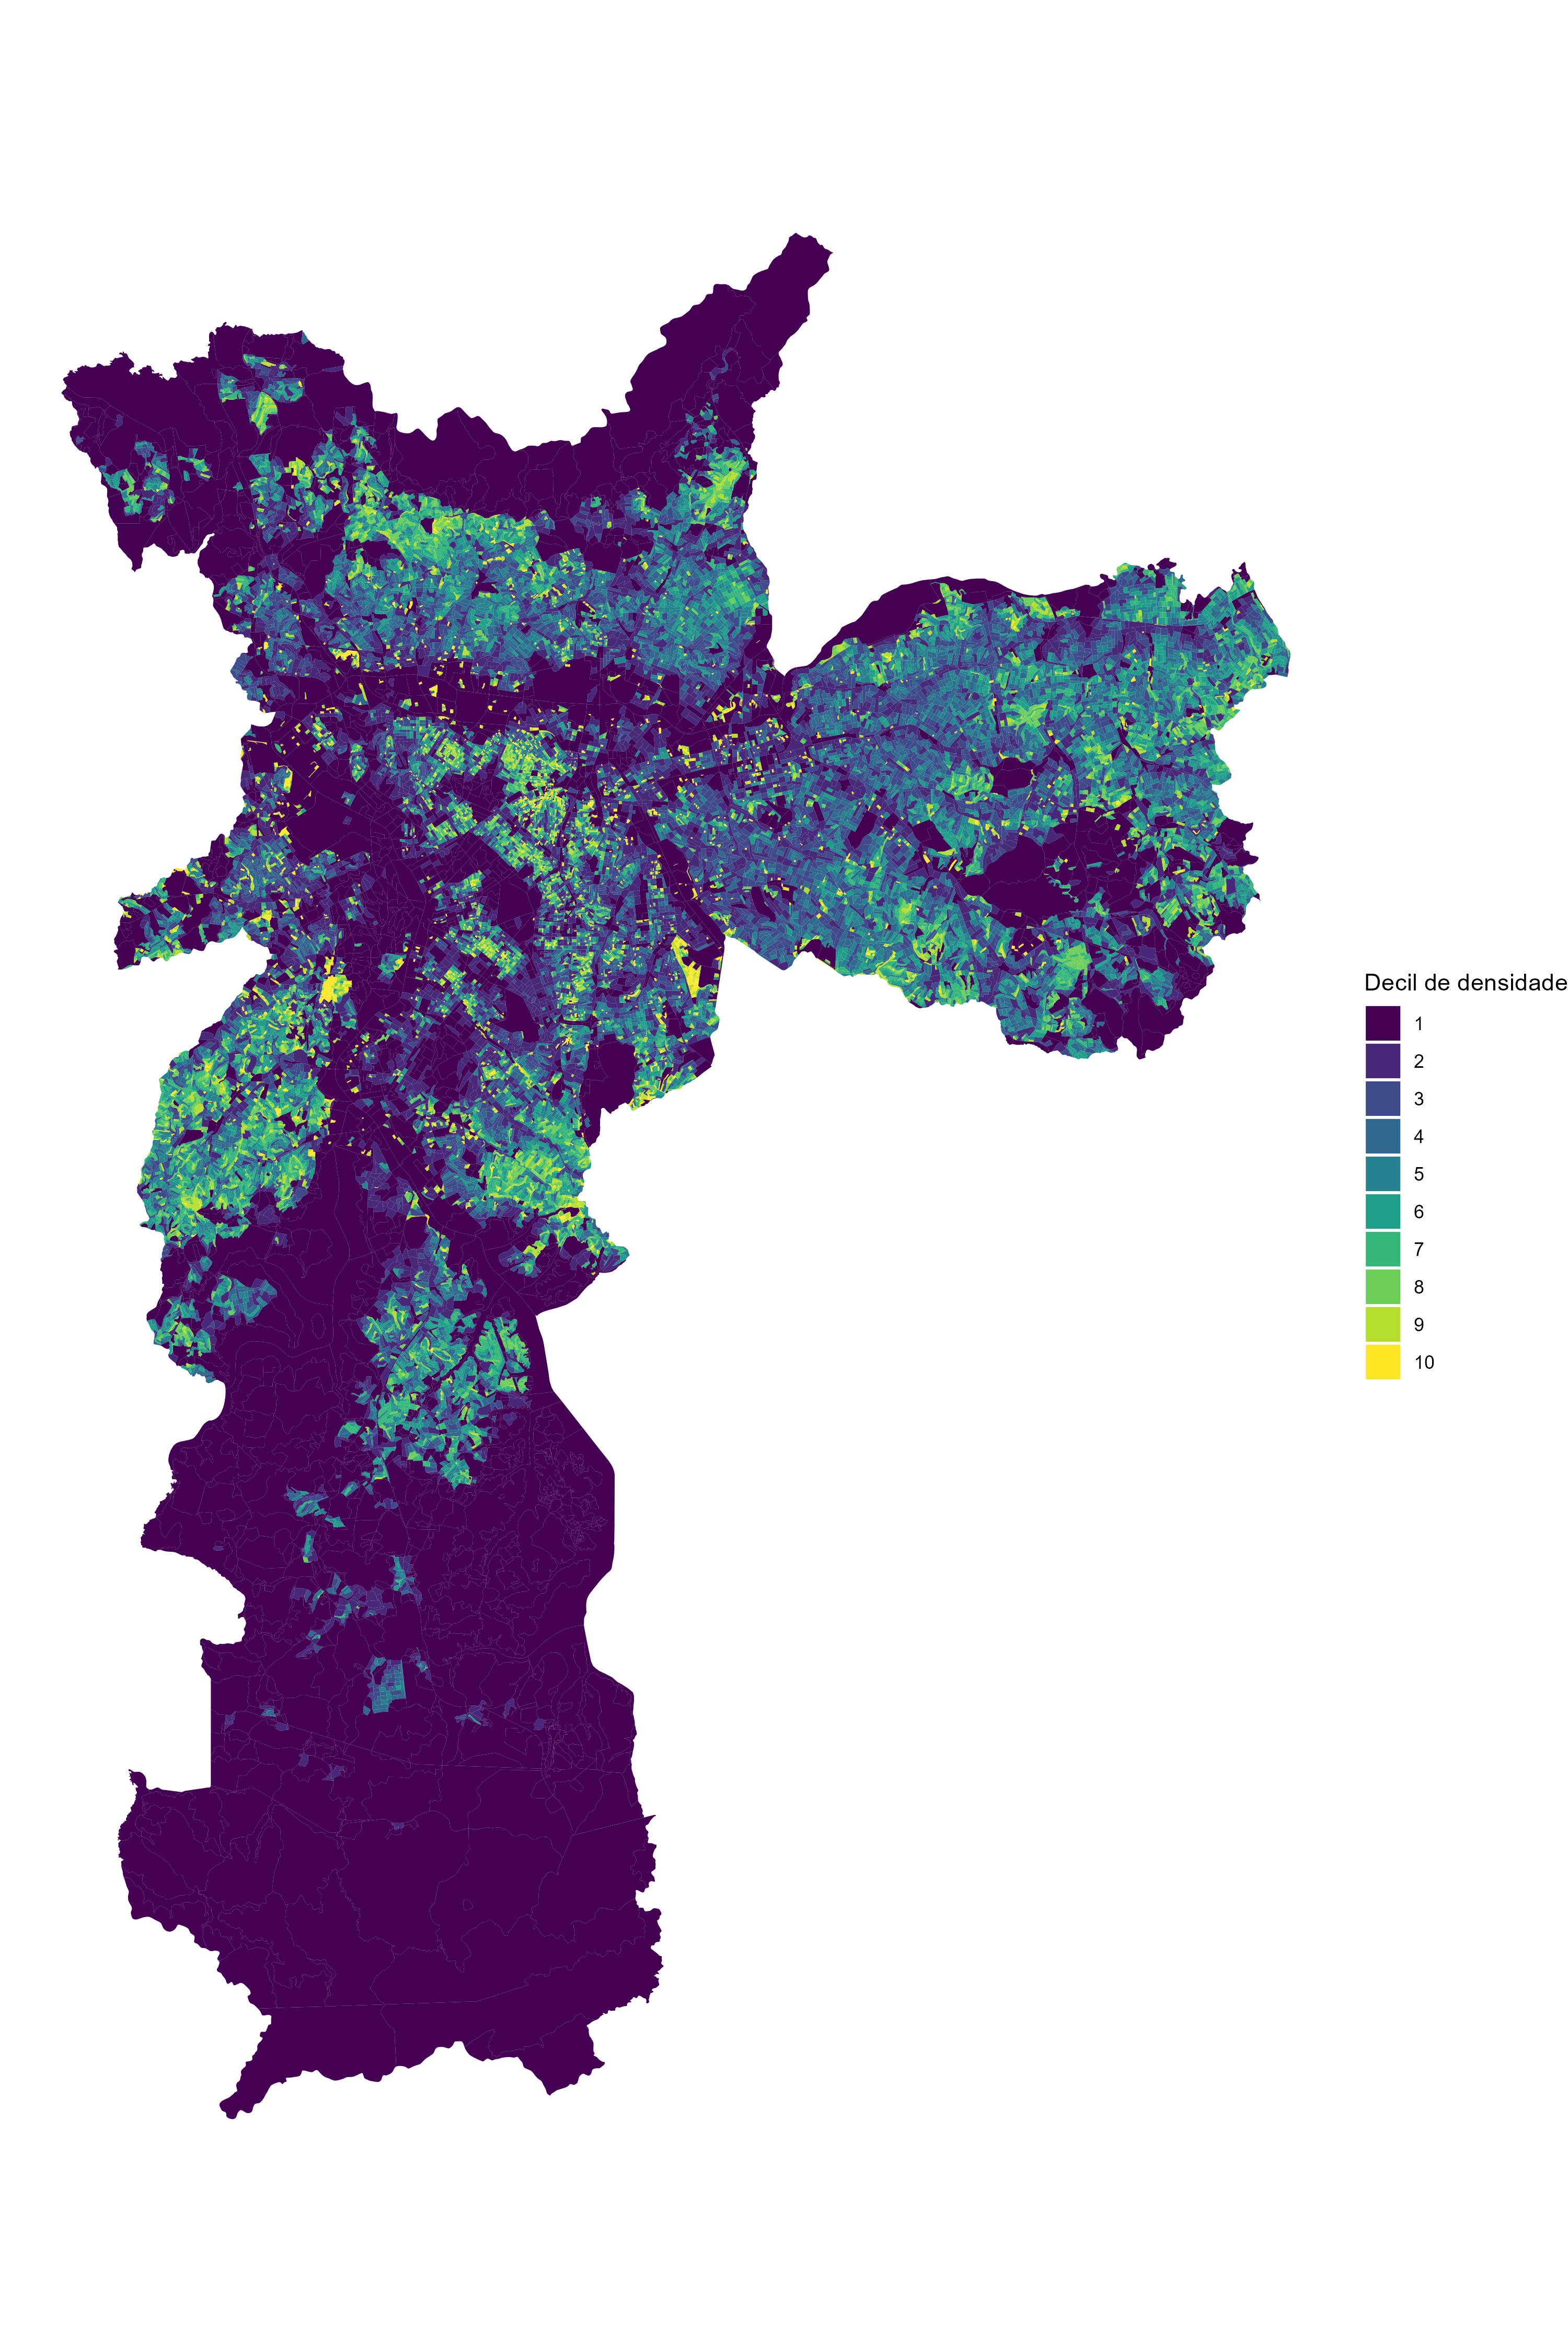
\includegraphics[width = \linewidth]{imagens/mapa.png}
    \label{fig:populacao}
\end{figure}

Em relação aos dados sobre os empreendimentos imobiliários, a base de dados escolhida foi do IPTU. Para os fins deste artigo, ela é a mais completa, visto que não representa um fluxo de novos imóveis construídos todos os anos como a base da Embraesp, mas apresenta um estoque imobiliário. Dito isso, estão cadastrados os 3.096.719 números únicos de contribuintes, que, segundo a definição da documentação dos dados no geosampa, ``A cada imóvel urbano corresponderá um número de inscrição no Cadastro Imobiliário Fiscal, entendendo-se como imóvel: I - a área de terreno, construído ou não, definida em matrícula do competente Serviço de Registro de Imóveis ou em transcrições ainda vigente.''.

Entre os dados disponíveis do IPTU, se destacam a área do terreno, a área construída, a área útil e o número de pavimentos do empreendimento. Logo, com estes dados é possível calcular os indicadores utilizados pela regulamentação do coeficiente de aproveitamento (CA), gabarito e cota parte. A cota parte especificamente também pode ser calculada através dos dados do censo apenas.

Todavia, os dados do IPTU não são georreferenciados, então desacompanhados de outros dados não é possível cruzá-los com censo. O que possibilita fazer essa junção é que o número único de contribuinte, também é o código do Setor, Quadra e Lote (SQL) que o empreendimento se encontra. Nesse sentido, é possível decompor o SQL e cruzar com a base de lotes do geosampa, que contém a geometria de cada  um dos 1.677.980 lotes da cidade. O que explica a diferença entre o número de lotes e número de números dos contribuintes são os lotes que contém um condomínio, que pode haver diversos números únicos de contribuintes em apenas um lote. 

Uma dificuldade que surge ao juntar os dados do Censo com os do IPTU, é que setores censitários podem cortar os lotes de forma que um lote pertença a mais de um setor. Sendo assim, alguma premissa deve ser adotada para que se classifique em qual setor o lote será contabilizado para os cálculos dos indicadores utilizados pela regulamentação. Na Figura \ref{fig:lote-censo} é possível observar os lotes coloridos de vermelho e os setores censitários coloridos como na Figura \ref{fig:populacao} e delimitados por um contorno branco. Quando um lote é cortado em mais de um setor censitário, é calculada a porcentagem de sua área em cada um dos setores e ele é contabilizado em ambos, ponderado por essa porcentagem.


\begin{figure}[h]
    \centering
    \caption{Lotes e setores censitários na Lapa}
    \includegraphics[width = \linewidth]{imagens/mapa-lotes.png}
    \label{fig:lote-censo}
\end{figure}

\postextual
\bibliography{bibliografia} 

% Apêndices
% \begin{apendicesenv}
%
% Imprime uma página indicando o início dos apêndices
% \partapendices



% \end{apendicesenv}



% Anexos

% \begin{anexosenv}
% 
% Imprime uma página indicando o início dos anexos
% \partanexos
% 
%
% \chapter{Capítulo anexo 1}


% \end{anexosenv}

% \bibliography{bibliografia}


% \begin{apendicesenv}

% % Imprime uma página indicando o início dos apêndices
%\partapendices

\end{document}